\documentclass[utf8,handout]{beamer}

\usepackage{presentation}
\title{Сервис поиска электронных книг}
\subtitle{Серверная часть, обеспечивающая хранение информации о~книгах, поиск по ней и возможность модифицировать её}

\author{Иваницкий Андрей}

\institute{Санкт-Петербургский Академический Университет РАН}
\date{\today}

\begin{document}

\begin{frame}
	\titlepage
	\begin{flushright}
    Руководитель: Николай Михайлович Пульцин

  \end{flushright}
\end{frame}

\section*{План презентации}
	\begin{frame}
		\frametitle{План презентации}
		\tableofcontents[pausesections]
	\end{frame}

\section{Введение}
\subsection{Описание проблемы}
  \begin{frame}

    \frametitle{Описание проблемы}
    \begin{enumerate}
      \item История (библиотеки, книжные магазины)
      \item Интернет (электронные библиотеки)
      \item Проблемы
	      \begin{itemize}
		    \item Проблема поиска
            \item Проблема единого интерфейса
            \item Проблема многих форматов книг
	      \end{itemize}
      \end{enumerate}
  \end{frame}

\subsection{Обзор существующих решений}
  \begin{frame}
    \frametitle{Обзор существующих решений}

    \begin{enumerate}
      \item Google books
      \item Проект eBdb
      \item Amazon Kindle, Sony Reader \\
			~
      \item OPDS
      \item BookServer
    \end{enumerate}
  \end{frame}


\subsection{Описание системы}
	\begin{frame}
		\frametitle{Описание системы в целом}
		OPDS --- The Open Publication Distribution System \\ 
~\\
~\\
		
\includegraphics{./head/scheme}
	\end{frame}

	\begin{frame}
		\frametitle{Описание внутренней структуры системы}
		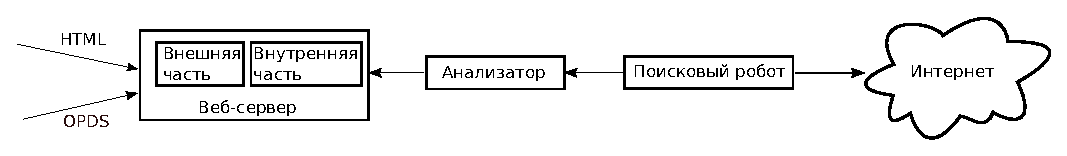
\includegraphics[width=1.05\textwidth]{./head/innerstructure}
	\end{frame}


\section{Постановка задачи}
	\begin{frame}
		\frametitle{Постановка задачи}
		\begin{enumerate}
			\item \textbf{Поиск по данным} \\
				Мощный, быстрый и удобный поиск как для пользователя, \\
				так и для анализатора.
			\item \textbf{Интерфейс модификации данных} \\
				Полный, гибкий и расширяемый интерфейс модификации~данных для анализатора.		
		\end{enumerate}
	\end{frame}


\section{Поиск по данным}
	\begin{frame}
 		\frametitle{Поиск по данным}
 		Реализовн поисковый механизм с помощью Sphinx
 		\begin{block}{}
			Предоставляет
			\begin{enumerate}
				\item  Релевантный поиск как по отдельным сущностям, так и по~различным их комбинациям;
				\item  Фильтрация результатов поиска по некоторым сущностям (язык книги, тэг);
				\item  Поиск с учётом морфологии языка;
				\item  Простой поиск (простой в использовании);
				\item  Исправление опечаток в запросе;
				\item  Поиск среди авторов по звучанию.
			\end{enumerate}
		\end{block}
	\end{frame}
	

\section{Интерфейс модификации данных}
	\subsection{Алгоритм взаимодействия с анализатором}
	\begin{frame}
 		\frametitle{Алгоритм взаимодействия с анализатором}
 		\begin{block}{}
	 		К каждой сущности добавлены два понятия:
 			\begin{enumerate}
 				\item {\em индекс доверия (credit)}
 				\item {\em индекс релевантности (relevance)}
 			\end{enumerate}
 		\end{block}
 		\begin{block}{}
			Если для автора {\em индекс доверия} и {\em релевантности} оказались \textbf{больше} пороговых значений, то
			\textbf{не~создаётся} новой сущности.\\
			В противном случае \textbf{создаётся} новый автор.\\
			~ \\
			Если для книги {\em индекс доверия} и {\em релевантности} оказались \textbf{больше} пороговых значений и
			авторы этой книги распознались как уже существующие в базе, то новой сущности \textbf{не~создаётся}.\\
			В противном случае \textbf{создаётся} новая книга.
		\end{block}
 	\end{frame}


	\subsection{Расчёт расстояния между строками}
	\begin{frame}
 		\begin{block}{Алгоритм: \textbf{Расчёт расстояния между строками}}
 			Две строки $s_{1}$ и $s_{2}$ разбиваются на слова:
 			$s_{1}\rightarrow S_{1}=\lbrace a_{1},\ldots,a_{n}\rbrace$, $s_{2}\rightarrow S_{2}=\lbrace b_{2},\ldots,b_{m}\rbrace$ \\
 			Пусть $n\leq m$

			$ M_{i,j} = D_{Levenshtein}(a_{i},b_{j}), i=1..n, j=1..m $ \\
			где $D_{Levenshtein}$ --- расстояние Левенштейна
			
			\[	C_{min}=\min_{\alpha_1, \alpha_2, \ldots, \alpha_m}{\sum_{i=1}^{n} M_{i,\alpha_{i}}} \] \\
			где $\alpha_1, \alpha_2, \ldots, \alpha_m$ --- перестановка чисел от $1$ до $m$,\\
			минимум по всем таким возможным перестановкам

			$C_{full}=C_{min}+(m-n)\times C_{remove}$\\
			где $C_{remove}$ --- цена добавления/удаления слова.
		\end{block}
	\end{frame}

	\subsection{Фаза добавления}
		\begin{frame}[fragile]
 			\frametitle{Структура запроса}
 			Запрос состоит из двух секций: {\em define}, {\em update}
 			\begin{block}{}
	 			\begin{verbatim}
<?xml version="1.0" encoding="UTF-8"?>
<request>
    <define>
        ...
    </define>

    <update>
        ...
    </update>
</request>
				\end{verbatim}
			\end{block}
		\end{frame}
	
		\begin{frame}[fragile]
 			\frametitle{Секция define}
  			Определяеются сущности с {\em уникальным идентификатором ui}
 			\begin{block}{}
	 			\begin{verbatim}
<author ui="1">
    <full_name> Leo Tolstoy </full_name>
</author>

<file ui="2">
    <link>http://example.com</link>
    <type>pdf</type>
    <size>4563214</size>
</file>
				\end{verbatim}
			\end{block}
		\end{frame}
	
		\begin{frame}[fragile]
 			\frametitle{Секция update}
 			Обновляются связи между сущностями
 			\begin{block}{}
	 			\begin{verbatim}
<book ui="3">
    <authors>
        <author id="343" />
        <author ui="1" />
    </authors>
    <files>
        <file ui="2" />
    </files>
</book>

				\end{verbatim}
			\end{block} 			
		\end{frame}
	
\section{Заключение}
	\begin{frame}
		\frametitle{Заключение}
		\begin{block}{}
			\begin{enumerate}
				\item Разработана внутренняя часть веб-сервера;
				\item С помощью Sphinx реализован мощный быстрый поиск;
				\item Реализован гибкий, расширяемый протокол взаимодействия с анализатором.
			\end{enumerate}
		\end{block}
		\begin{block}{}
		Полная работающая система доступна в Интернете по адресу\\ \url{http://ebooksearch.webfactional.com/} \\
		~\\
		Исходный код проекта в репозитории google\\ \url{http://code.google.com/p/ebooksearchtool/}
		\end{block}
	\end{frame}
	




\end{document}
